\documentclass[a4paper,12pt,fleqn]{article}
\usepackage{fixltx2e}
\usepackage[utf8]{inputenc}
\usepackage{graphicx}
\usepackage{sidecap}
\usepackage{fancyhdr}
\usepackage{amssymb,amsmath}
\usepackage[swedish]{babel}
\usepackage[margin=1.5in]{geometry}
\usepackage{abstract}
\usepackage[parfill]{parskip}
\usepackage{tocloft}
\usepackage{adjustbox}
\usepackage{textcomp}
\usepackage[T1]{fontenc}
\usepackage{listings}
\usepackage{xcolor,colortbl}
\usepackage{hyperref}

%----------------------------------------------------------------
%C-kod formatering

\definecolor{listinggray}{gray}{0.9}
\definecolor{lbcolor}{rgb}{0.9,0.9,0.9}
\lstset{
backgroundcolor=\color{lbcolor},
    tabsize=4,    
%   rulecolor=,
    language=[GNU]C++,
        basicstyle=\scriptsize,
        upquote=true,
        aboveskip={1.5\baselineskip},
        columns=fixed,
        showstringspaces=false,
        extendedchars=false,
        breaklines=true,
        prebreak = \raisebox{0ex}[0ex][0ex]{\ensuremath{\hookleftarrow}},
        frame=single,
        numbers=left,
        showtabs=false,
        showspaces=false,
        showstringspaces=false,
        identifierstyle=\ttfamily,
        keywordstyle=\color[rgb]{0,0,1},
        commentstyle=\color[rgb]{0.026,0.112,0.095},
        stringstyle=\color[rgb]{0.627,0.126,0.941},
        numberstyle=\color[rgb]{0.205, 0.142, 0.73},
%        \lstdefinestyle{C++}{language=C++,style=numbers}’.
}
\lstset{
    backgroundcolor=\color{lbcolor},
    tabsize=4,
  language=C++,
  captionpos=b,
  tabsize=3,
  frame=lines,
  numbers=left,
  numberstyle=\tiny,
  numbersep=5pt,
  breaklines=true,
  showstringspaces=false,
  basicstyle=\footnotesize,
%  identifierstyle=\color{magenta},
  keywordstyle=\color[rgb]{0,0,1},
  commentstyle=\color{Darkgreen},
  stringstyle=\color{red}
  }
  %-----------------------------------------------------------------
  %marginaler

  \renewcommand{\abstractnamefont}{\normalfont\normalsize\bfseries}
  \renewcommand{\abstracttextfont}{\normalfont\small}
  \renewcommand{\headrulewidth}{0pt}
  \renewcommand{\cftsecleader}{\cftdotfill{\cftdotsep}} 
  \setlength{\absleftindent}{0pt}
  \setlength{\absrightindent}{0pt}
  \setlength{\headheight}{15pt}

  \addtolength{\oddsidemargin}{-.5in}
  	\addtolength{\evensidemargin}{-.5in}
  	\addtolength{\textwidth}{1in}


  %-----------------------------------------------------------------
  %header and footer

  \pagestyle{fancy}
  \lhead{
  	\begin{picture}(0,0)
  		\put(5,0){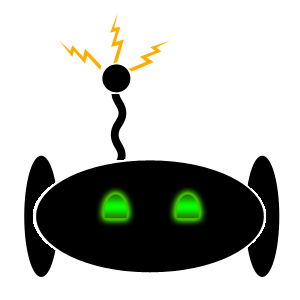
\includegraphics{logotyp.png}}
  	\end{picture}}
	
  \fancyhead[C]{\small{Mapmaster2001}}
  \fancyhead[R]{\small \today}
  \fancyfoot[L]{\small{TSEA56 \\ LIPS Kappa}}
  \fancyfoot[C]{\small{\thepage}}
  \fancyfoot[R]{\small{Projektgrupp 8 \\ mapmaster2001@cyd.liu.se}}

  %-----------------------------------------------------------------

%-------------------------------------------------------------------
%Första sidan

\begin{document}
	\pagestyle{fancy}
\pagenumbering{roman}
	\vspace*{\fill}
		\begingroup
			\begin{center}
				\huge{\textbf{Teknisk dokumentation}}
				\\
				\vspace{5pt}
				\normalsize
				Kandidatprojekt Y - Grupp 8 - VT2014
				\\
				Version 1.0
				\end{center}
		\endgroup
	\vspace*{\fill}
	
	\begin{center} %Börjar centrering 
		Status
		\\
		\vspace{3pt} %Whitespace 3 pts
	    \begin{tabular}{| p{3cm} | p{3cm} | p{3cm} |} %tabell, 4 horizontella |, 3 cm emellan dem.
	    \hline %översta horizontella linjen.
	    Granskad & NE,TG & \today \\ \hline % & -tecken för att "gå till nästa ruta" 
		Godkänd & - & - \\ \hline % avslutas med \\ och \hline.

	    \end{tabular}
	\end{center}
	\vspace{2cm}
	\newpage
%-----------------------------------------------------------------
%Projektidentitet
	
	\vspace*{\fill}
		\begingroup
			\begin{center}
				\LARGE{\textbf{PROJEKTIDENTITET}}
				\\
				\footnotesize
				Grupp 8, 2014/VT, MapMaster2001
				\\
				Linköpings tekniska högskola, ISY
				\\
				\vspace{1cm}
	  \begin{tabular}{| p{3cm} | p{4.3cm} | p{2.4cm} | p{3.8cm} |}
	    \hline
		\textbf{Namn} & \textbf{Ansvar} & \textbf{Telefon} & \textbf{E-post} \\ \hline
	    Jens Edhammer & Dokumentanvsvarig (DOK) & 076-030 67 80 & jened502@student.liu.se \\ \hline
		Erik Ekelund & Designansvarig (DES) & 073-682 43 06 & eriek984@student.liu.se \\ \hline
		David Habrman &  & 976-017 71 15 & davha227@student.liu.se \\ \hline 
		Tobias Grundström & Testansvarig (TES) & 073-830 44 45 & tobgr602@student.liu.se \\ \hline 
		Hans-Filip Elo &   & 073-385 22 32 & hanel742@student.liu.se \\ \hline 
		Niklas Ericson & Projektledare (PL) & 073-052 27 05 & niker917@student.liu.se \\ \hline
	    \end{tabular}
		
		\vspace{1cm}
		\textbf{E-postlista för hela gruppen:} mapmaster2001@cyd.liu.se
		\\[0.5cm]
		
		\textbf{Kund}: Mattias Krysander, Linköpings Universitet, 581 83  LINKÖPING, \\
		013-28 21 98, matkr@isy.liu.se \\
		\textbf{Kontaktperson hos kund}: Mattias Krysander, 013-28 21 98,matkr@isy.liu.se 
		\\
		\textbf{Kursansvarig}: Tomas Svensson, 3B:528,013 28 21 59,tomass@isy.liu.se
		\\[0.5cm]
		\textbf{Handledare}: Peter Johansson, 013-28 1345 peter.a.johansson@liu.se

				\end{center}
		\endgroup
	\vspace*{\fill}
\newpage

%-----------------------------------------------------------------
%Innehållsföreteckning

\addto\captionsswedish{\renewcommand{\contentsname}{Innehållsförteckning}}

\tableofcontents
\thispagestyle{fancy}
\newpage

\pagenumbering{arabic}

%-----------------------------------------------------------------
%Översikt

\section{Inledning} 
Bakgrund och syfte. 

\section{Produkt}
En bild på produkten och en beskrivning av hur den fungerar.
Beskriv vad den används till.

\section{Teori}
Beskrivning av regleralgoritmer mm.

%-----------------------------------------------------------------
%Systemet
\section{System}

\begin{figure}[htp] %Placera här om det finns plats, annars så snart som möjligt, på toppen av en sida.
  \begin{center}
  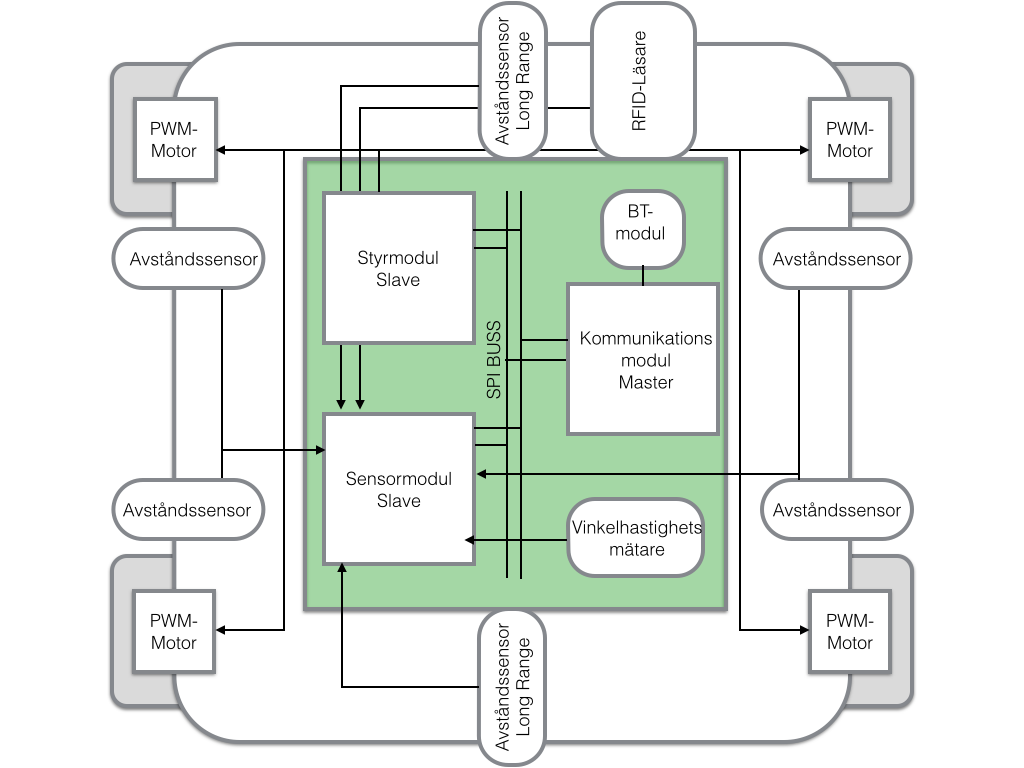
\includegraphics[keepaspectratio=true,width=\linewidth]{bilder/overview}  %skala och filnamn. 
  \end{center}
  \caption{Översiktsbild av systemet} %figurtext.
  \label{fig:overview}
\end{figure}

\subsection{Ingående delsystem}
Roboten består av tre delsystem, en buss, ett chassi samt en tillhörande mjukvara för persondator. Sensormodulen kommer att hantera analoga sensorsignaler samt omvandla dessa till användbart mätdata som skickas vidare tll kommunikationsmodulen. 
Kommunikationsenheten kommer att agera master och därav sköta all kommunikation mellan de andra enheterna. Kommunikationsmodulen sköter även kommunikationen mellan mjukvaran och roboten via en bluetoothadapter. Styrenheten kommer sköta robotens fyra drivande motorer, kartlägga samt ta beslut om körriktning vid autonom operation.
De tre delsystemen kommer att kommunicera via en SPI-buss och är byggda runt processorerna ATMEL Atmega 1284p med 16KByte SRAM som är fullt tillräckligt för att kunna använda C++ och en objektorienterad programmeringsstruktur.

Chassit kommer vara i storlkesordningen 30cm och ha fyra PWM-motorer, placerade på längst fram och längstbak på sidorna av chassit. Motorerna kommer att vara fixa i chassit, vilket betyder att roation kommer utföras genom att införa en rotationshastighetsdifferens mellan motorparen.

Sensorerna som tillhör sensormodulen kommer alla, förutom robotens tillhörande RFID-läsare, att vara symetriskt utplacerade på chasit. Två långdistanssensorer av typ GP\-2Y\-3A\-00\-3K\-0F placerade centrerat i fram och bak på roboten kommer användas för odometri. Ovanför varje däck plaseras en medeldistanssensor som kommer användas för att upptäcka sidokorridorer samt för att reglera roboten vid färd.
I fronten kommer även en RFID-läsare för upptäckt av de RFIDmarkerade brandhärdena placeras och kretskortet för modulerna kommer ett gyro för mätning av vinkelhastighet att placeras. Denna kommer användas för att bedöma orientering av roboten.

\subsection{Kommunikation via buss}
En buss med protokoll SPI kommer att sköta kommunikationen mellan robotens tre delsystem. SPI-protokollet är ett fullt-duplext kommunikationsprotokoll som fungerar genom att byta 8 lokala bitar med 8 bitar från modulen den kommunicerar med. 

Ett eget konstruerat dataprotokoll kommer implementeras. Protokollet är konstruerat så att de 4 högsta bitarna som skickats in på registret specificerar vilket kommando som skickas.
De följande 4 anger hur många cykler, dvs. hela Bytes som datat som skickas i samband med kommandot kommer upta. 0x**00 kommer tolkas som att en Byte ska skickas vilket inebär att Datamängden som kan skickas per kommando har 17*8 bitar som tak.

\begin{figure}[htp] %Placera här om det finns plats, annars så snart som möjligt, på toppen av en sida.
  \begin{center}
  \includegraphics[keepaspectratio=true,width=\linewidth]{bilder/bussprotokoll}  %skala och filnamn. 
  \end{center}
  \caption{Översiktsbild av bussprotokollet} %figurtext.
  \label{fig:bussprotocol}
\end{figure}


% ----------------------------- Kommunikationsmodul ------------------------------
% --------------------------------------------------------------------------------


\section{Kommunikationsmodul}
Modul för att hantera kommunikation mellan robotens olika delkomponenter samt med persondatorn via Blåtand. Kommunikationsmodulen som syns i figur 3, kommer att agera master på robotens interna buss. Vid kommunikation mellan övriga moduler, dvs. sensor- och 'en, kommer denna gå via kommunikationsmodulen.
Kommunikationsmodulen kommer alltså att leverera sensordata mellan roboten och mjukvaran som körs på persondatorn.

\begin{figure}[htp] %Placera här om det finns plats, annars så snart som möjligt, på toppen av en sida.
  \begin{center}
  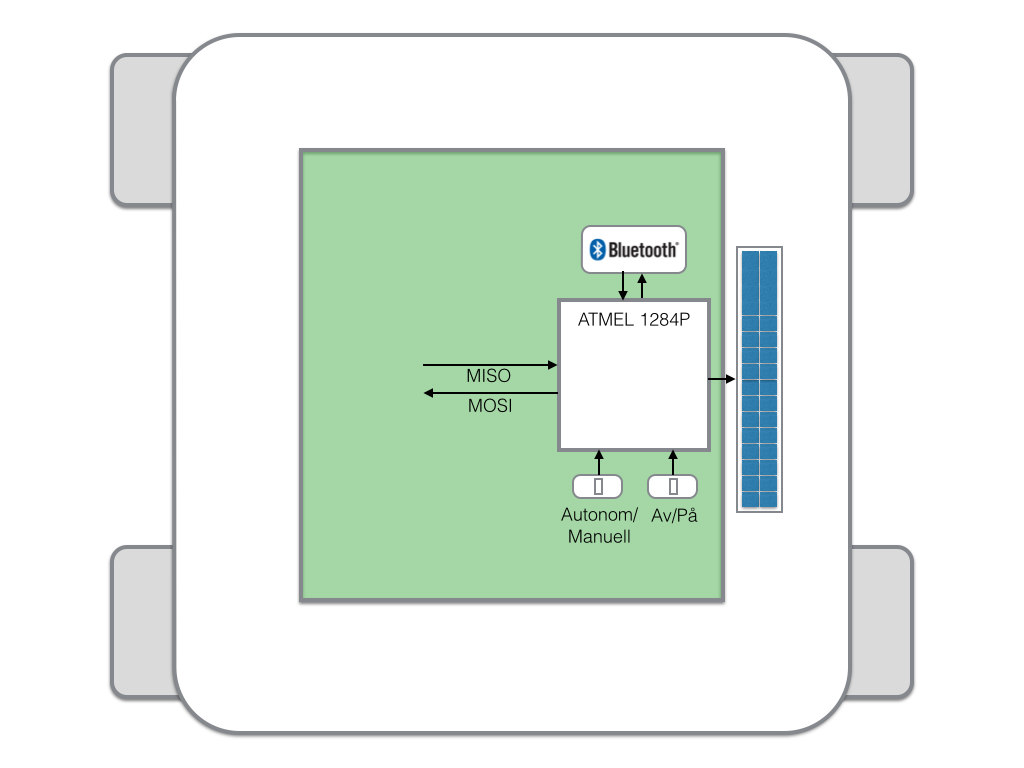
\includegraphics[keepaspectratio=true,width=\linewidth]{bilder/komoverview.png}  %skala och filnamn. 
  \end{center}
  \caption{Översiktsbild av kommunikationsdelen av systemet} %figurtext.
  \label{fig:overview}
\end{figure}

\subsection{Kommunikationsfall}
Ett par exempel på kom\-mun\-ikations\-fall.

Kommunikationsmodulen skickar data mellan de olika enheterna. Ett par olika kommunikationsfall demonstreras i flödesdiagramm i Appendix B.

Fall 1: Kommunikationsmodulen skickar manuella styrkommandon till styrmodulen, se figur~\ref{fig:case1flow}.

Fall 2: Sensormodulen signalerar att ny sensordata är redo, se  figur~\ref{fig:case2flow}.

Fall 3: Kartdata skickas från kommunikationsmodulen till PC, se figur~\ref{fig:case3flow}. 

Fall 4: PC signalerar nödstop, se figur~\ref{fig:case4flow}. 

 
\subsection{Komponenter}
\begin{itemize}
  \item AVR processor av typen ATMega1284
  \item Blåtandsdongel, Firefly, BlueSmirf Gold
  \item LCD-Display
  \item Två stycken knappar
  \item Kristalloscillator EXO-3, 14.745 MHz
\end{itemize}

\subsection{Buss}
Mellan processorerna kommer SPI-kommunikation att användas. Kommunikationsmodulen agerar master medan styr- och sensormodul agerar slave. 

\subsubsection{Styrord}
Kommunikation kommer starta med att ett styrord skickas. Ett styrord kommer bestå av ett 8-bitars paket (xxxxyyyy). De fyra mest signifikanta bitarna står för kommandot medan de 4 minst signifikanta bitarna står för antalet byte som kommer att följa som argument till kommandot. I tabellerna nedan visas detta mer utförligt. \\

 \begin{tabular}{| p{3cm} | p{3.5cm} |}
	    \hline
		\textbf{xxxx} & \textbf{Kommandonr.} \\ \hline
		0000 & 1 \\ \hline
		0001 & 2 \\ \hline
		... & ... \\ \hline
		1111 & 17 \\ \hline
	    \end{tabular}
		\\

 \begin{tabular}{| p{3cm} | p{3.5cm} |}
	    \hline
		\textbf{yyyy} & \textbf{Antal bytes data} \\ \hline
		0000 & 1 \\ \hline
		0001 & 2 \\ \hline
		... & ... \\ \hline
		1111 & 17 \\ \hline
	    \end{tabular}
		\vspace{0.5cm}
		
		Detta betyder alltså att master kan skicka 16 unika kommandon till respektive slave och varje slave kan skicka 16 unika kommandon till master. Kommandon kan följas av ett upp till och med 17 bytes av data. I händelsen att ett meddelande inte behöver skicka data så skickas en byte nollor.


		Kommandon kommer att kunna betyda olika på de olika processorerna. 0001 kan t ex på slave1 betyda åk rakt längs väggen, på slave2 betyda läs av sensor 3, och på master uppdatera kartabstraktion med följande värden. Om likadana kommandon finns på flera processorer så ska de ha samma kodord på alla processorer som delar kommandot. Ett kommando är reserverat på båda slaves för ett kommando från master som säger du kan skicka information nu. En slave kommer också att kunna skicka ett avbrott till Master för att be om kommunikation. En lista av de olika kodorden finns i appendix. 
		
På både mottagar- och sändarsida kommer en buffer i form av en länkad lista finnas. Denna lista fylls med data som tas emot och läses från när data ska skickas. 


\subsubsection{Busstrafik}
På bussen kommer följande data att skickas.
\paragraph{Styrkommandon från PC}
~\\
När styrkommandona skickas från PC, kommer kommunikationsmodulen skicka datat vidare till styrmodulen som utför kommandot.
\paragraph{Konverterat sensordata}
~\\
Sensordata kommer att behandlas i sensormodulen och därefter kommer modulen att skicka ett avbrott till master om att data finns tillgängligt. Mastern svarar och startar bussöverföringen.
\paragraph{Kartabstraktion så styrenheten kan välja färdväg}
~\\
Kartabstraktionen och robotens position kommer att uppdateras allt eftersom ny sensordata kommer in. Efter att ny sensordata har  mottagits av masters, skickar mastern ut sensordata till styrenheten.
\paragraph{Kommandon för inställning av reglerparametrar.}
~\\
Kommandon mottags via blåtand från PC på mastern, som skickar detta vidare till styrenheten. 


\subsubsection{Ack-paketets struktur}
Ett sista paket som följer direkt efter datapaketen kommer att skickas. Detta paket är ack-paketet och kommer vara additionen av samtliga datapaketets lägsta bit. Detta ger mottagarsidan en möjlighet att kontrollera att datapaketen mottogs korrekt.
Både sändaren och mottagaren skickar ett sådant ack-paket samtidigt, detta ger oss möjlighet att göra om sändningen direkt, utan att lämna ett eventuellt avbrott. Försök att skicka data utförs tre gånger, om det fortfarande inte lyckats skicka korrekt data, avbryts försöken och lämnas över till felhantering. 

\subsection{LCD-Display}
Sensordata och annan information från roboten kommer att visas på en alfanumerisk-display, närmare bestämt  LCD JM162A. Displayen kommer att kunna visa 2 rader × 16 tecken.
Displayen kommer anslutas till processorn enligt kretschemat i appendix A. 
Vid varje uppstart kommer initiering av LCD-display göras och då följa nedanstående flödesschema. Varje steg startas med att processorn skickar ett kommando till ingångarna på LCD-displayen. Kommandon finns specificerade i databladet, se (fotnot https://docs.isy.liu.se/twiki/pub/VanHeden/DataSheets/jm162a.pdf). 

\subsubsection{Uppstart}
	
Vid uppstart av systemet kommer LCD-displayen att initieras enligt flödes\-schemat~\ref{fig:flowlcdstart}

\begin{itemize}
  \item Power ON - sätter på strömförsörjningen
  \item Function set - Sätter överförsdatalängden till 8 bitar och displayläget till 2-rader.
  \item Display ON - slår på displayen och slår på markören. 
  \item Entry mode set - sätter markörens riktning vid skrivning
  \item End - Slut på initieringen
\end{itemize}

\begin{figure}[htp]
	  \begin{center}
	  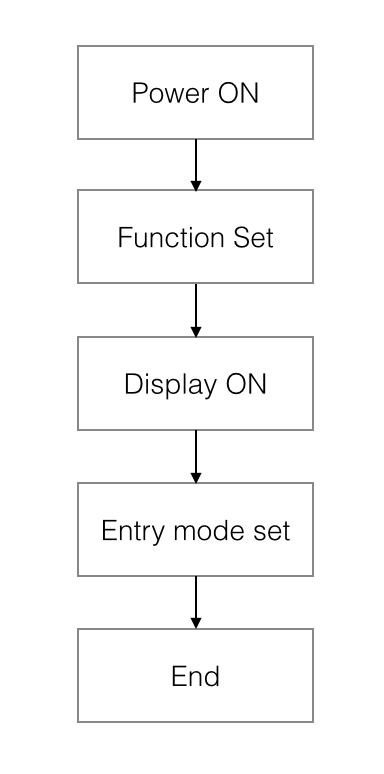
\includegraphics[keepaspectratio=true,scale=0.4]{bilder/startup}  %skala och filnamn. 
	  \end{center}
	  \caption{Uppstart av LCD-display} %figurtext.
	  \label{fig:flowlcdstart}
	\end{figure}

\newpage


\subsubsection{Skrivning}

Vid skrivning till LCD-displayen kommer detta ske enligt flödesschemat~\ref{fig:flowlcdwrite}
\begin{itemize}
  \item Start write procedure - Startar skrivning till LCD-displayen
  \item Clear - Rensar hela displayen
  \item Set DDRAM - gör DDRAMet tillgängligt
  \item Write data to RAM - Skrivning av data in till RAM ifrån DDRAM
\end{itemize}

\begin{figure}[htp] %Placera här om det finns plats, annars så snart som möjligt, på toppen av en sida.
  \begin{center}
  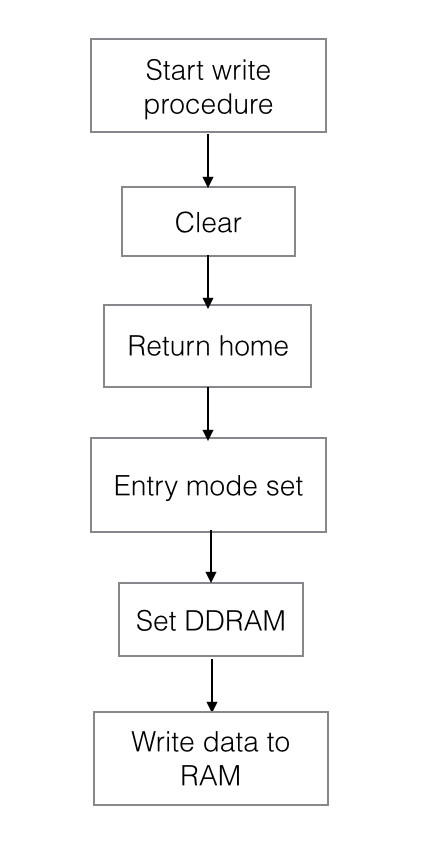
\includegraphics[keepaspectratio=true,scale=0.4]{bilder/write}  %skala och filnamn. 
  \end{center}
  \caption{Skrivning till LCD-display} %figurtext.
  \label{fig:flowlcdwrite}
\end{figure}

\subsection{Blåtand}
Blåtandskommunikationen kommer att utföras av ett Firefly-Bluesmirf gold (FBG) modem som parkopplas mot en persondator.
FBG kommer att skicka information till persondator via protokollet RS232 enligt vad som är angivet på Vanheden. 
Se schema i appendixet Scheman för anslutning av TxD och RxD, vilka sköter sändning och mottagning av data.
\subsection{Switchar}
En switch ska styra om roboten exekverar programkod för autonom styrning eller manuell styrning. Ett avbrott signalerar till processorn att den ska byta programkod, avbrottet ligger på pin16 (INT0) se appendix A. 
Av/På-knappen styr strömförsörjningen till samtliga moduler. 

% ----------------------------- Styrmodul --------------------------------------
% --------------------------------------------------------------------------------

\newpage
\section{Styrmodul}
Styrmodulens (slave) huvudkomponent kommer  att bestå av en AVR-processor, Atmel ATmega1284p som får instruktioner från kommunikationsmodulen (master) via bussen. Processorn kommunicerar även med drivkretsen på chassit. Chassit är av typen Terminator som drivs av en NiMH- eller NiCd-ackumulator på 7.2V. Det har även fyra stycken växlade DC-motorer som är kopplade till varsitt drivhjul. 

\begin{figure}[htp] %Placera här om det finns plats, annars så snart som möjligt, på toppen av en sida.
  \begin{center}
  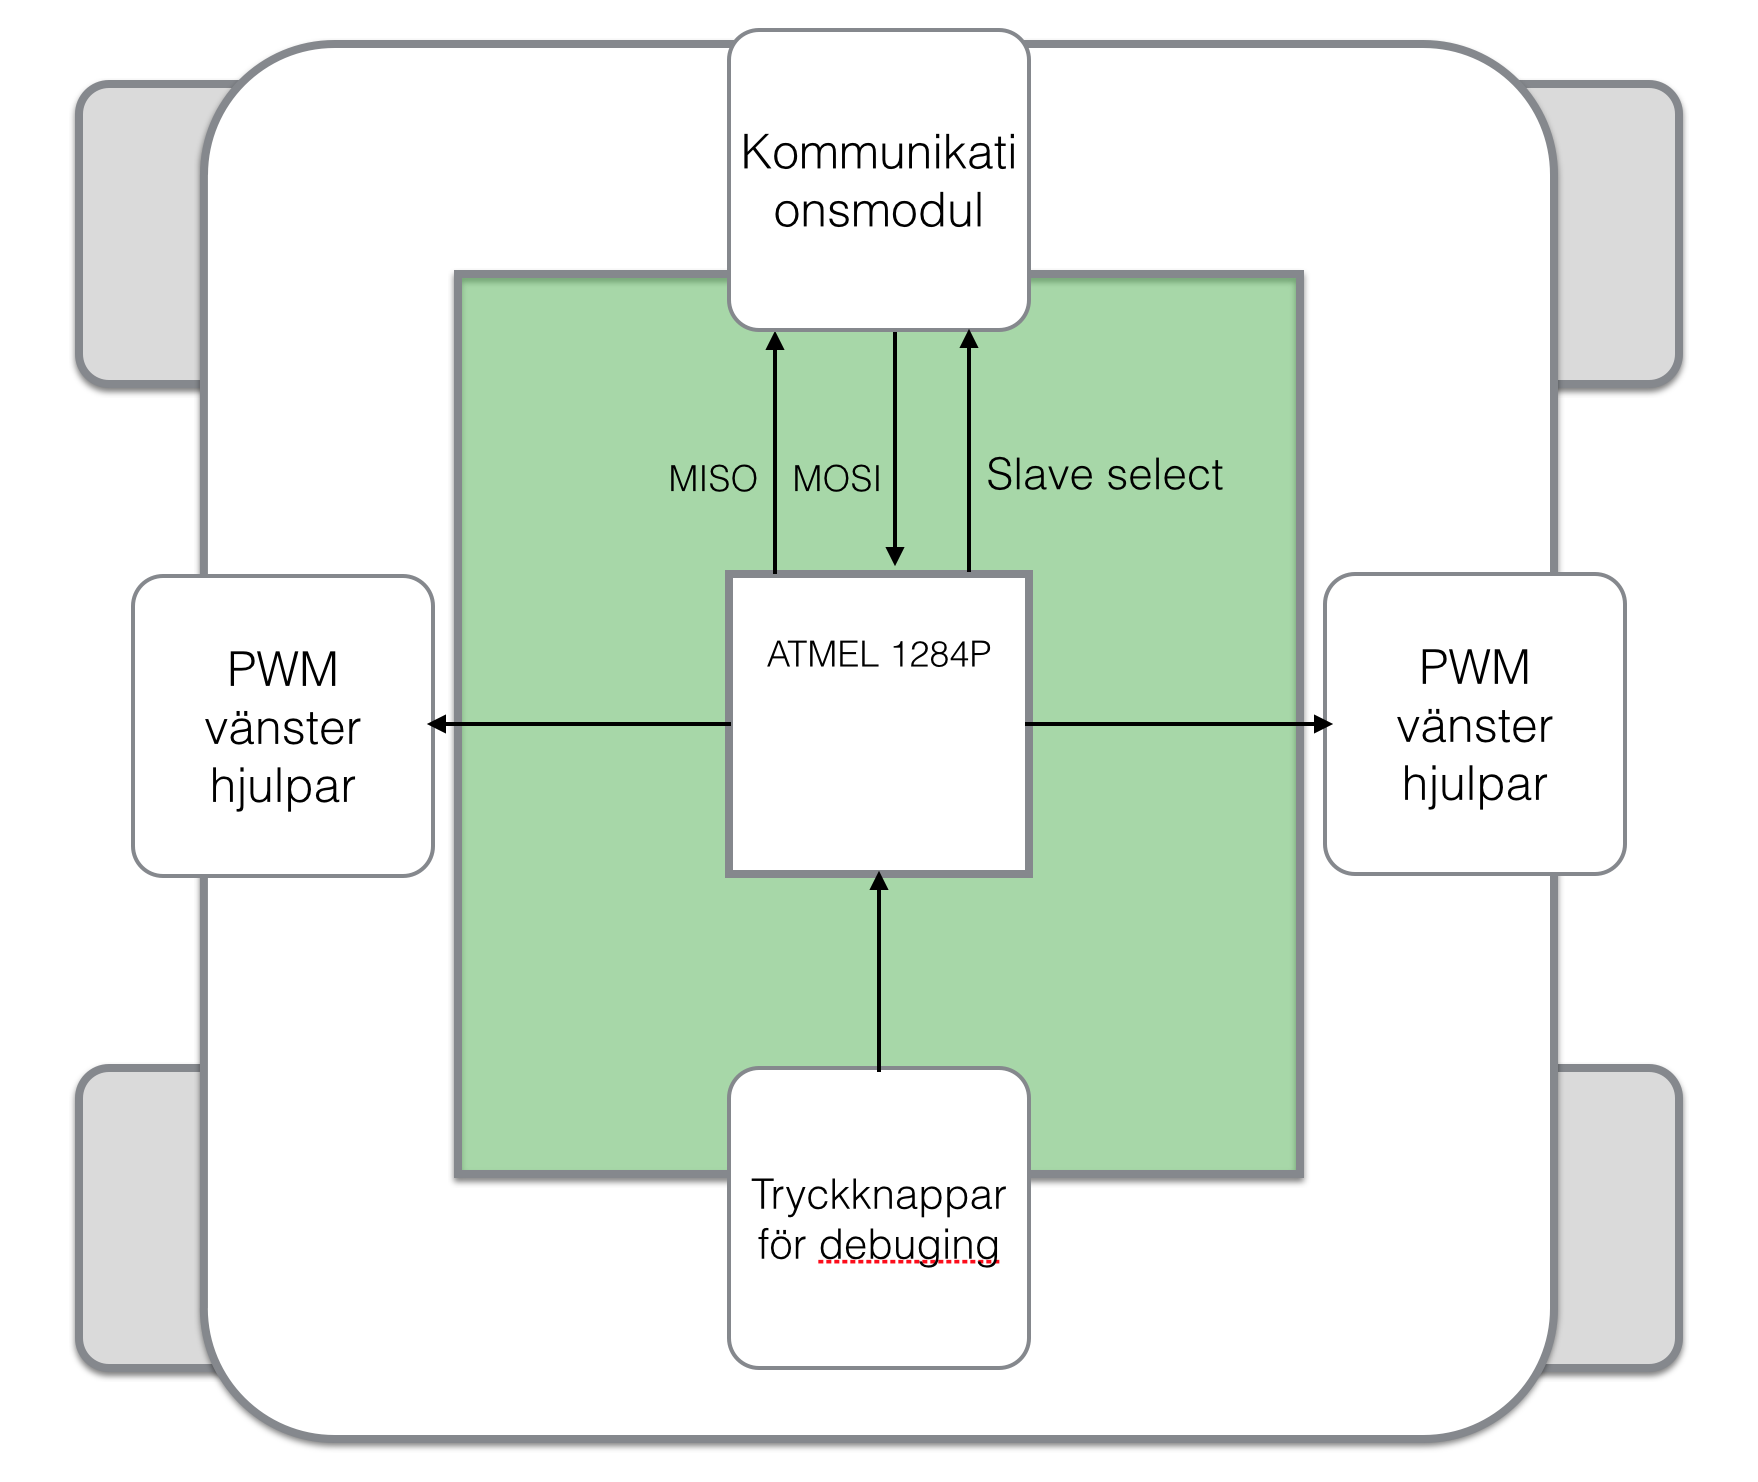
\includegraphics[keepaspectratio=true,scale=0.5]{bilder/styrmodul}  %skala och filnamn. 
  \end{center}
  \caption{Översikt styrmodul} %figurtext.
  \label{fig:styr} %glöm inte att uppdatera era labels
\end{figure}
\newpage

% ----------- Komponenter ------------------

\subsection{Komponenter}
\begin{itemize}
	\item Chassi
	\item Systemchip - Atmel ATmega1284p
	\item Tryckknappar för debugging av styrfunktionalitet
	\item Batteri, 7.2 V
	\item Resetknapp
\end{itemize}
~\\
Motorerna kommer att styras parvis med två signaler per sida:
\begin{itemize}
	\item DIRL - Styr den vänstra motorns rotationsriktning
	\item DIRR - Styr den högra motorns rotationsriktning
	\item PWML - Pulsbreddmodulerad signal som styr den vänstra motorns hastighet
	\item PWMR - Pulsbreddmodulerad signal som styr den högra motorns hastighet.
\end{itemize}
~\\
Dessa kopplas direkt från processorn till chassits drivkrets enligt bild.
Styrmodulen kommer att vara ansluten till bussen med hjälp av MISO- och MOSI-pinnarna.

\begin{itemize}
	\item MISO - Master Input Slave Output, data skickas till master
	\item MOSI - Master Output Slave Input, data skickas till slave
	\item MASTERINT - Skickar avbrott till master
	\item SLAVESELECT - Väljer denna processor som aktiv slav
	\item SCK - Serial Clock, klocka från master
\end{itemize}
~\\
Utöver detta kommer en tryckknapp anslutas till RESET för att förhindra att felaktig programmering av processorn. 

För fullständigt kopplingsschema - se Appendix. 

\newpage
% ------------------- Styrning och kartläggning -----------------------

\subsection{Styrning och kartläggning}
Det ska implementeras två olika avsökningsalgoritmer. De kommer användas beroende på vilket uppdrag roboten ska genomföra. Algoritmerna kommer att skrivas med hjälp av C++ och köras från processorns interna minne. 

\subsubsection{Kartläggninsalgoritm}

Kartläggningsalgoritmen utformas så att roboten börjar med att placera sig så att en vägg går att finna på höger sida. Roboten kommer sedan följa väggen till dess att den kan rita upp ett slutet område att arbeta utifrån. Nästa steg blir att kartlägga områden som ännu ej är kartlagda. Om en köksö upptäcks kommer roboten se till att rita upp hela köksön innan den går vidare. På detta sätt fortsätter algoritmen till dess att alla delar av rummet är kartlagda. 

\begin{figure}[htp] %Placera här om det finns plats, annars så snart som möjligt, på toppen av en sida.
  \begin{center}
  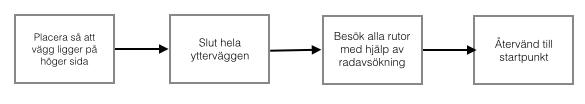
\includegraphics[keepaspectratio=true,scale=0.5]{bilder/flode_brandhard.jpg}  %skala och filnamn. 
  \end{center}
  \caption{Flödesschema kartläggningsalgoritm} %figurtext.
  \label{fig:map} %glöm inte att uppdatera era labels
\end{figure}

\newpage

\subsubsection{Brandhärdssökning}

Brandhärdssökningen kommer att gå till på liknande sätt som kartläggningsalgoritmen, dock kommer den vara långsammare på grund av att varje ruta i området måste besökas. Efter att området slutits använder roboten sig av radavsökning för att systematiskt besöka alla rutor. Om en RFID-tag upptäcks ska detta noteras.

\begin{figure}[htp] %Placera här om det finns plats, annars så snart som möjligt, på toppen av en sida.
  \begin{center}
  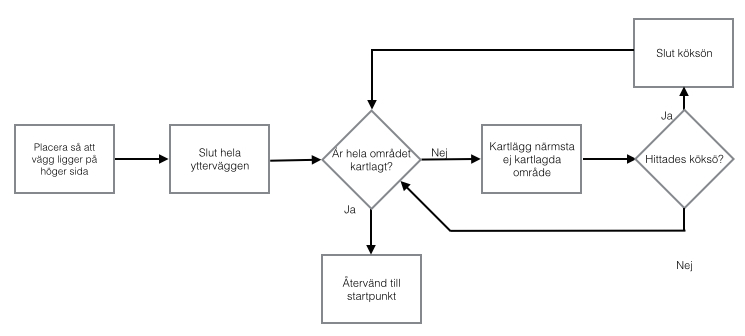
\includegraphics[keepaspectratio=true,scale=0.5]{bilder/Flode_kartritning.jpg}  %skala och filnamn. 
  \end{center}
  \caption{Flödesschema brandhärdssökning} %figurtext.
  \label{fig:fire} %glöm inte att uppdatera era labels
\end{figure}


\subsubsection{Kartabstraktion}
Kartan kommer att abstraheras som en matris där objekt sparas. Objektklasserna kommer att ha en moderklass med namn MapSection de sedan ärver från. Tillgängliga underklasser kommer att vara:

\begin{itemize}
\item{EmptySection}
\item{UnexploredSection}
\item{Robot}
\item{UnreachableSection}
\item{Fire}
\end{itemize}

\paragraph{EmptySection} 
~\\
EmptySection kommer att representera en tom sektion av kartan. Objektet EmptySection kan svara på frågan om huruvida den eller andra EmptySection som angränsar till ojektet i fråga i sin tur angränsar till outforskat område. 

\paragraph{UnexploredSection} 
~\\
UnexploredSection kommer att representera en outforskad sektion av kartan. 

\paragraph{Robot} 
~\\
Robot kommer att representera robotens position på kartan. 

\paragraph{UnreachableSection} 
~\\
Unreachable section kommer att representera ett block på kartan som är inringat av väggar. Dessa block kommer kunna svara på om de representerar ett slutet område och även om de angränsar till outforskat område. 

\paragraph{Fire} 
~\\
Fire kommer att representera plats där det finns eldhärd. 
\newpage
% ------------------- Reglering -----------------------

\subsection{Reglering}

Roboten kommer kunna styras dels autonomt men också manuellt via PC-mjukvara. 

\subsubsection{PD-reglering av styrning}
Styrmodulen kommer att få sensordata skickad till sig från sensormodulen. Denna sensordata kommer att användas till att PD-reglera riktningen då man följer en vägg. 

Den proportionella delen av regleringen kommer fås från avståndet till vägg vid sidan av roboten. 

$ e_p = K_{p}*avst\text{\it{å}}ndssensordata $

Där K är en konstant- Den deriverande delen av regleringen kommer ges av linjär uppskattning av derivatan utefter de senaste mätvärdena. Derivatan ges alltså av: 

$ e_d = K_{D}*(data/antal_sampels) $

Totala felet ges då av: 

$e = e_d + e_p$


% ----------- Kommunikation ------------------

\subsection{Kommunikation}

Styrmodulen kommunicerar med kommunikationsmodulen (master) över en SPI-buss. Bussen kopplas in på dedikerade pinnar för SPI-bussen på ATmega1284p-processorn. Kommunikationsmodulen kommer att agera master på bussen. 

De kommandon styrmodulen kommer att kunna hantera beskrivs i tabellen nedan. \newline

\begin{tabular}{| p{0.25\textwidth} | p{0.15\textwidth} | p{0.075\textwidth} | p{0.075\textwidth} | p{0.35\textwidth} |}
	\hline
	\rowcolor{listinggray}
	\textbf{Funktion} & \textbf{Kommando} & \textbf{Från} & \textbf{Till} & \textbf{Förklaring} \\ \hline
	Nödstopp & 0x00 & Komm & Styr & Stanna alla motorer \\ \hline
	Autonom styrning & 0x01 & Komm & Styr & Aktivera PD-reglering och styralgoritmer \\ \hline
	Manuell styrning & 0x02 & Komm & Styr & Avaktivera PD-reglering och styralgoritmer \\ \hline
	Framåt & 0x03 & Komm & Styr & Kör framåt \\ \hline
	Bakåt & 0x04 & Komm & Styr & Kör bakåt \\ \hline
	Vänster & 0x05 & Komm & Styr & Sväng vänster \\ \hline
	Höger & 0x06 & Komm & Styr & Sväng höger \\ \hline
	Sensordata & 0x07 & Komm & Styr & Ta emot sensordata från master \\ \hline
	Sätt reglerkonstanter & 0x08 & Komm & Styr & Sätter värden för konstanter till PD-reglering \\ \hline
\end{tabular}

\newpage


% ----------------------------- Sensormodul --------------------------------------
% --------------------------------------------------------------------------------

\section{Sensormodul}
Sensor modulen kommer ha till uppgift att hantera sensordata från robotens 8 sensorer och sända detta vidare till com-delen i ett hanterbart format. Sensormmdulen är byggd kring AVR-processorn ATMEL 1284p. En överblick av systemet visas i figur~\ref{fig:sensoroverview}.

\begin{figure}[htp] %Placera här om det finns plats, annars så snart som möjligt, på toppen av en sida.
  \begin{center}
  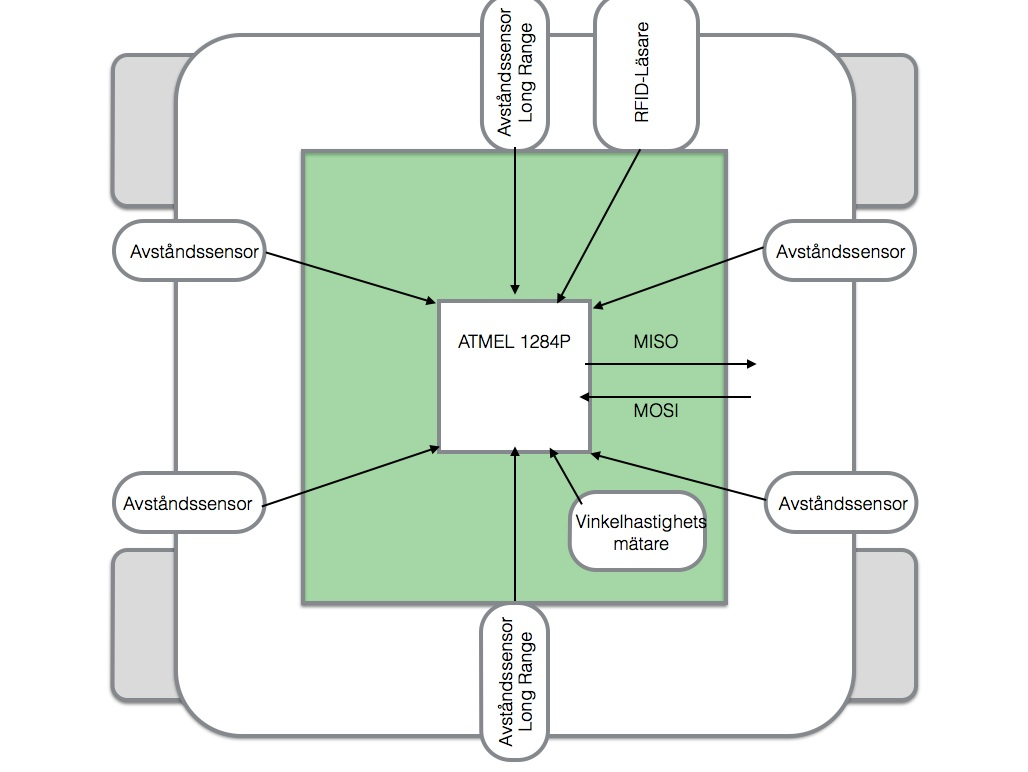
\includegraphics[keepaspectratio=true,width=\linewidth]{bilder/overblicksensor}  %skala och filnamn. 
  \end{center}
  \caption{Överblick av sensormodulen} %figurtext.
  \label{fig:sensoroverview}
\end{figure}

\subsection{Kopplingsschema}

En beskrivande bild av kopplingsschemat finns i appendix A.

Port A användas som en A/D-omvandlare. PIN 39-40 kopplas till avståndssensorer för långdistans, GP\-2Y\-3A\-00\-3K\-0F, PIN 35-38 kopplas till avståndssensorer för kortdistans, GP\-2Y\-0A\-21\-YK, och PIN 34 kopplas till ett gyro för vinkelhastighetsmätning, ML\-X9\-06\-09. Port B används för busskommunikation. PIN 3 skickar avbrott till master, PIN 5 används till slave select master, PIN 6 tar emot data från bussen, PIN7 skickar data till bussen och till PIN 8 kopplas klockan från master. Till port C PIN 23 kopplas en RFID-läsare, Parallax-Reader. Port D används inte i denna modul. 

PIN 31 och 11 kopplas till jord, PIN 13 kopplas till klocka från master, PIN 12 används inte i denna modul, PIN 9 kopplas till en avstudsad manuell switch, en resetknapp, PIN 32 kopplas till en spänningskälla på 5 V som används som referensspänning, PIN 10 kopplas också den till en spänningskälla på 5 V och PIN 30 kopplas genom ett LP-filter till samma externa spänningskälla.

\subsection{Uppgift}
Sensormodulens uppgift är att A/D-omvandla signaler från robotens avståndssensorer, RFID-sensor och gyro för att sedan utnyttja dessa digitala värden för att uppskatta avstånd, tillryggalagd sträcka och positionering. I figur~\ref{fig:sensorflow} beskrivs hanteringen av sensordata.

\begin{figure}[htp] %Placera här om det finns plats, annars så snart som möjligt, på toppen av en sida.
  \begin{center}
  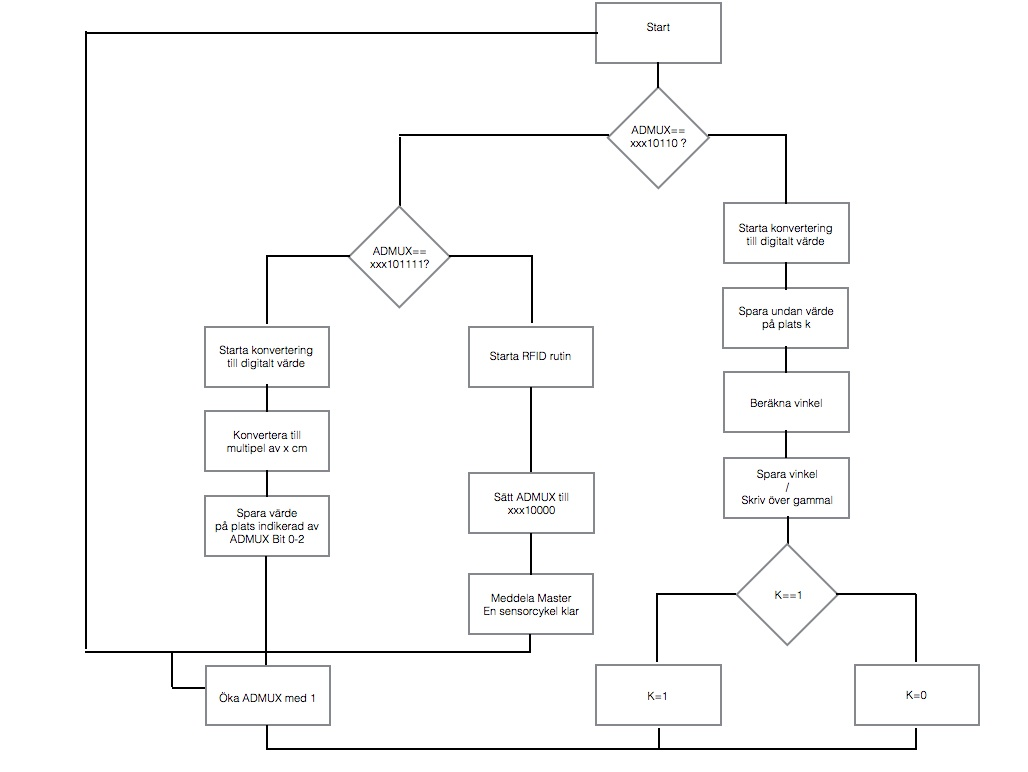
\includegraphics[keepaspectratio=true,width=\linewidth]{bilder/sensorflode}  %skala och filnamn. 
  \end{center}
  \caption{Flödesdiagram för sensorhantering} %figurtext.
  \label{fig:sensorflow}
\end{figure}

\subsection{Komponenter}
\begin{itemize}
	\item Systemchip - Atmel ATmega1284p
	\item RFID-sensor - Par\-all\-ax-Read\-er\
	\item 2 st avståndssensorer för längre avstånd - GP\-2Y3A\-00\-3K\-0F
	\item 4 st avståndssensorer för kortare avstånd - GP\-2Y\-0A\-21\-YK
	\item Vinkelhastighetssensor - MLX\-90\-609
\end{itemize}
~\\

\subsubsection{Systemchip}
Modulens processor är av typen Atmel ATmega1284p\footnote{http://www.atmel.com/ja/jp/Images/doc8059.pdf}. Processorn kommer kontinuerligt att ta in data från alla sensorer. Denna är programmerbar och kommer att innehålla de program som behövs för att konvertera signalerna till avstånd, tillryggalagd sträcka, positionering och detektion av RFID-tagg. På begäran av master, kommunikationsmodulen, kan data skickas från processorn till master via en SPI-buss.

\subsubsection{RFID-sensor}
För att kunna detektera RFID-taggen så krävs en sensor. Vi kommer att använda Par\-all\-ax-Read\-er\footnote{https://docs.isy.liu.se/twiki/pub/VanHeden/DataSheets/rfid-reader-v21.pdf}. 
SOUT på RFID-sensorn, PIN 3, kopplas till port C, PIN 23, på processon. RFID-taggen skickar alltså sin data till processorn för behandling.

Brus kan ge upphov en falsk RFID-läsning. För att ungå detta problem accepteras läsningen endast om två på varandra följande läsningar ger samma utslag på RFID-läsaren. Det är väldigt osannolikt att brus skulle ge upphov till exakt samma signal under två på varandra följande läsningar.

\subsubsection{Avståndssensorer}
Roboten kommer att ha sex stycken av\-stånds\-sensorer varav två är för lång\-distans, GP\-2Y3A\-00\-3K\-0F 40-300 cm som går att läsa om på Vanheden\footnote{https://docs.isy.liu.se/twiki/pub/VanHeden/DataSheets/gp2y3a003k0f.pdf}  och resterande 4 är för \hyphenation{kort-dist-ans},GP\-2Y\-0A\-21\-YK 10-80 cm som finns på Vanheden\footnote{https://docs.isy.liu.se/twiki/pub/VanHeden/DataSheets/gp2y0a21.pdf}. En av långdistanssensorerna placeras fram på roboten och den andra bak. De fyra kortdistanssensorerna placeras två stycken på vardera sida.

PIN 6 på långdistanssensorerna och PIN 1 på kortdistanssenorerna kopplas till port A, PIN 39-40, respektive port A, PIN 35-38, på processorn. Sensorerna skickar alltså sin data till processorn för A/D-omvandling och tolkning.

GND på sensorerna sätts till jord, Vcc och Vin sätts till hög och PIN 3 på långdistanssensorerna sätts till hög.
 
Data från sensorerna behövs för att detektera väggar och skapa en kartabstraktion. Data från sensorerna för långdistans används dessutom för att beräkna tillryggalagd sträcka medans sensorerna på sidan används för att reglera roboten under färd.

\subsubsection{Vinkelhastighetssensor (gyro)}
För att underlätta beräkningar av körriktningar och hålla koll på hur mycket roboten svängt används en vinkelhastighetssensor eller gyro, MLX\-90\-609 på Vanheden \footnote{https://docs.isy.liu.se/twiki/pub/VanHeden/DataSheets/MLX90609\_datasheet.pdf}. OUTAR på gyron, PIN 24, kopplas direkt till bussen för att minska brus. Gryot skickar en spänning mellan 0.5 och 4.5 V där 2.5 V motsvarar vinkelhatsighet noll.

Vinkelberäkning kommer ske med följande formel: \newline
$ a(k) = a(k-1)+0.5T(\delta a(k)+\delta a(k-1))$ \\
Där $a(k)$ är nuvarande sampels vinkel, $\delta a(k)$ är vinkelhastighet i nuvarande sampeln, $a(k-1)$ är förra sampelns beräknade vinkel, $\delta a(k-1)$ är vinkelhastigheten i förra sampeln och T är samplingstiden.

\subsubsection{Övriga komponenter}
Övriga komponenter så som ett batteri på 7.2 V och en resetknapp kommer att användas till denna modul.

\subsection{Övergripande design}
Sensorerna kommer att vara placerade engligt bilden i figur~\ref{fig:sensoroverview} .

\section{Slutsatser}
Vilka förbättringar skulle kunna göras?

\section{Referenser}



% ----------------------------- Appendix -----------------------------------------
% --------------------------------------------------------------------------------

\newpage
\appendix
\pagestyle{empty}
\newgeometry{left=2cm,right=2cm,bottom=2cm,top=2cm}
\section{Appendix A - Kopplingsscheman}
\subsection{Kopplingsschema för kommunikationsmodul}

\begin{figure}[ht] %Placera här om det finns plats, annars så snart som möjligt, på toppen av en sida.
  \begin{center}
  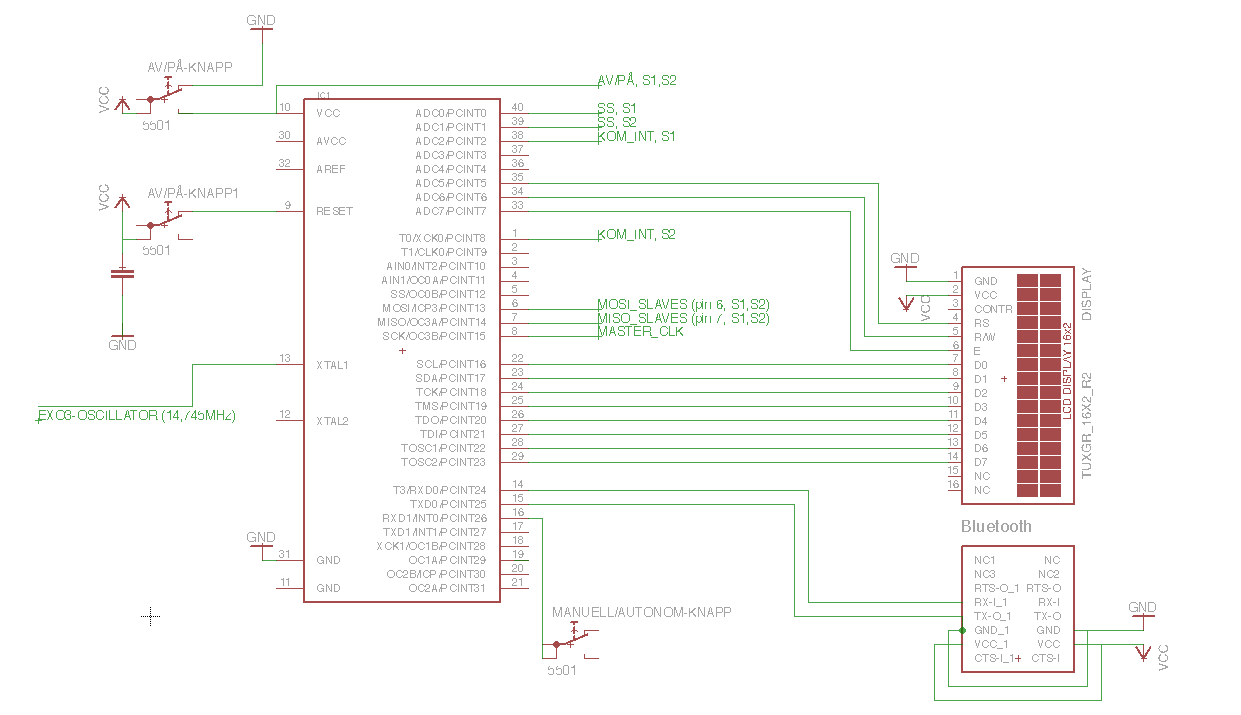
\includegraphics[keepaspectratio=true,width=\linewidth]{bilder/komschema.png}  %skala och filnamn. 
  \end{center}
  \caption{Kopplingsschema kommunikationsmodul} %figurtext.
  \label{fig:kopplingkom} %glöm inte att uppdatera era labels
\end{figure}
 \clearpage %flushes picture cache to place now
 

\subsection{Kopplingsschema för styrmodul}

\begin{figure}[ht] %Placera här om det finns plats, annars så snart som möjligt, på toppen av en sida.
  \begin{center}
  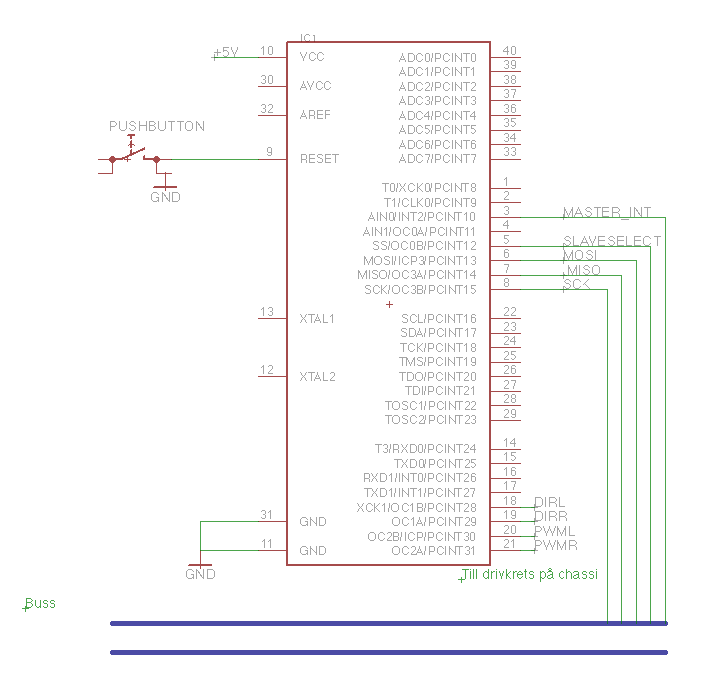
\includegraphics[keepaspectratio=true,width=\linewidth]{bilder/kopplingsschema_styrmodul.png}  %skala och filnamn. 
  \end{center}
  \caption{Kopplingsschema styrmodul} %figurtext.
  \label{fig:kopplingstyr} %glöm inte att uppdatera era labels
\end{figure}
 \clearpage %flushes picture cache to place now
 

\subsection{Kopplingsschema för sensormodull}

\begin{figure}[ht] %Placera här om det finns plats, annars så snart som möjligt, på toppen av en sida.
  \begin{center}
  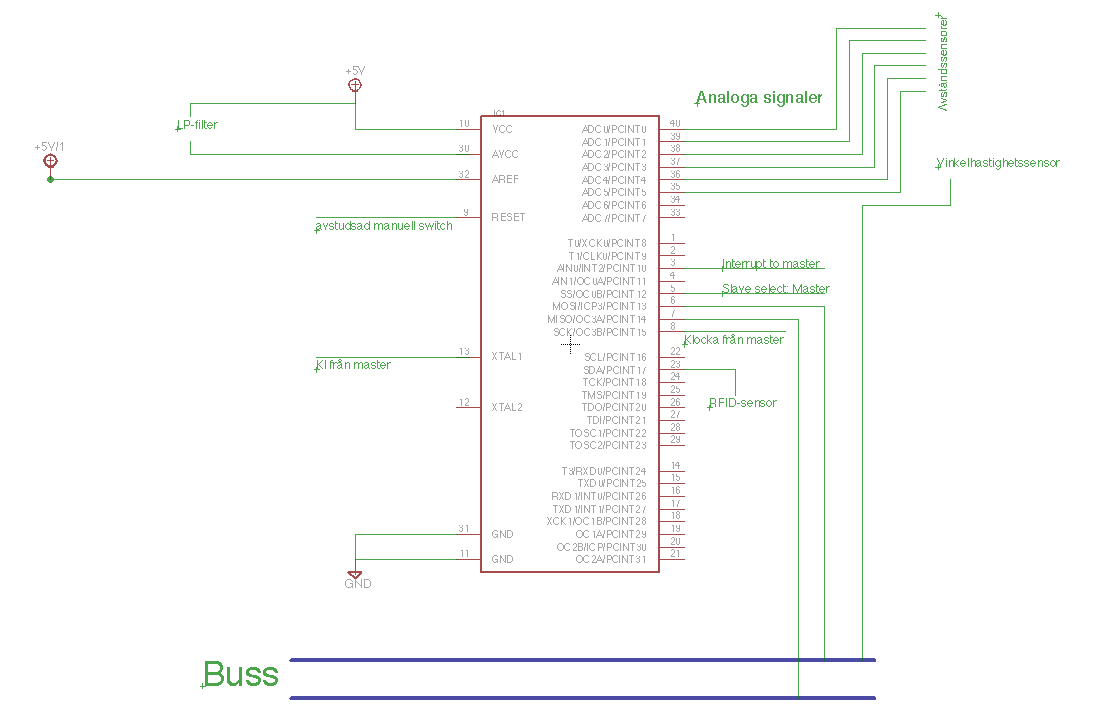
\includegraphics[keepaspectratio=true,width=\linewidth]{bilder/sensormodulkoppling.png}  %skala och filnamn. 
  \end{center}
  \caption{Kopplingsschema sensormodul} %figurtext.
  \label{fig:kopplingsensor} %glöm inte att uppdatera era labels
\end{figure}
 \clearpage %flushes picture cache to place now
 

\newpage
\section{Appendix B - Flödesscheman}

\begin{figure}[htp] %Placera här om det finns plats, annars så snart som möjligt, på toppen av en sida.
  \begin{center}
  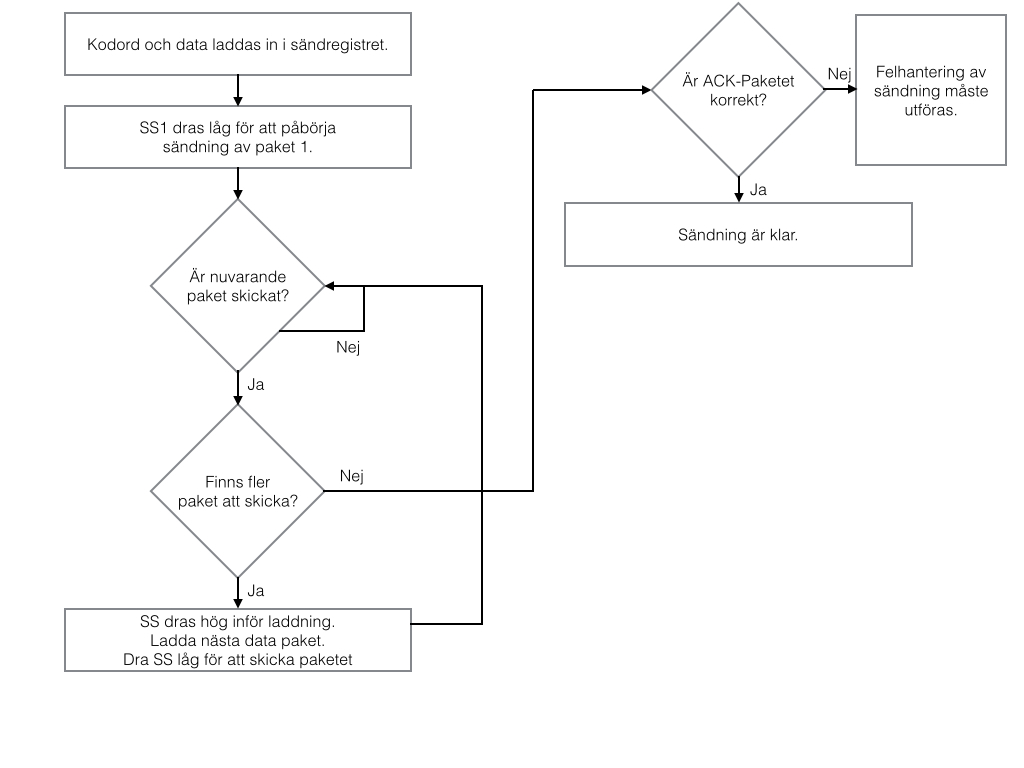
\includegraphics[keepaspectratio=true,width=\linewidth]{bilder/SPIbild002.jpg}  %skala och filnamn. 
  \end{center}
  \caption{Flödesdiagram för Fall 1.} %figurtext.
  \label{fig:case1flow}
\end{figure}

\begin{figure}[htp] %Placera här om det finns plats, annars så snart som möjligt, på toppen av en sida.
  \begin{center}
  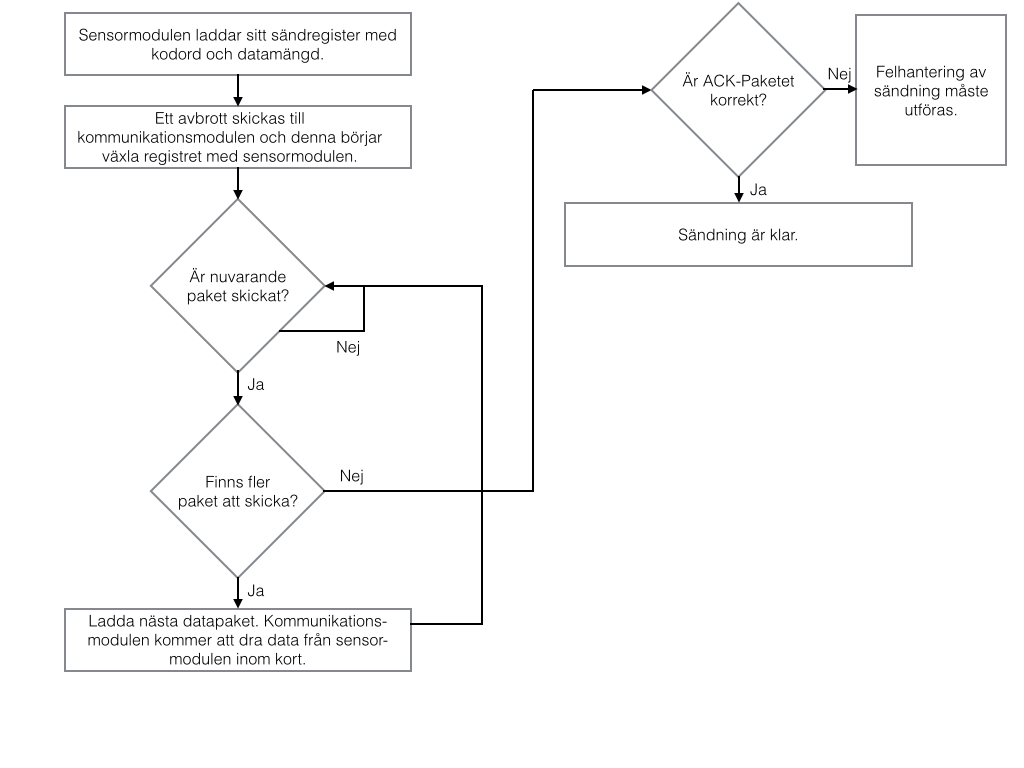
\includegraphics[keepaspectratio=true,width=\linewidth]{bilder/SPIbild003.jpg}  %skala och filnamn. 
  \end{center}
  \caption{Flödesdiagram för Fall 2.} %figurtext.
  \label{fig:case2flow}
\end{figure}
\begin{figure}[htp] %Placera här om det finns plats, annars så snart som möjligt, på toppen av en sida.
  \begin{center}
  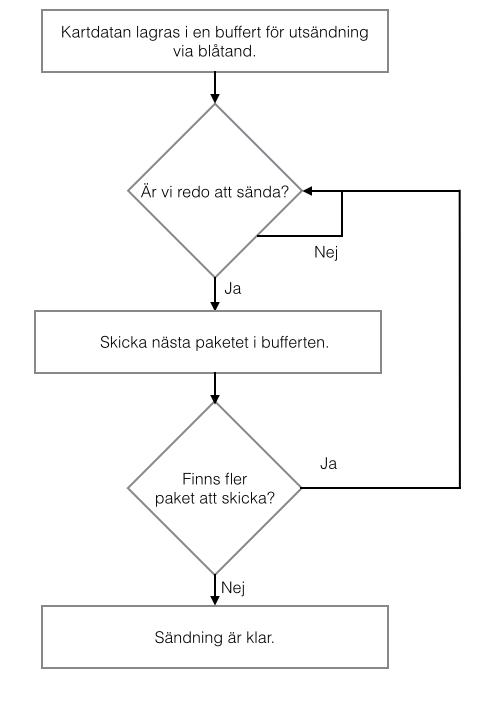
\includegraphics[keepaspectratio=true,width=0.9\linewidth]{bilder/SPIbild004.jpg}  %skala och filnamn. 
  \end{center}
  \caption{Flödesdiagram för Fall 3.} %figurtext.
  \label{fig:case3flow}
\end{figure}
\begin{figure}[htp] %Placera här om det finns plats, annars så snart som möjligt, på toppen av en sida.
  \begin{center}
  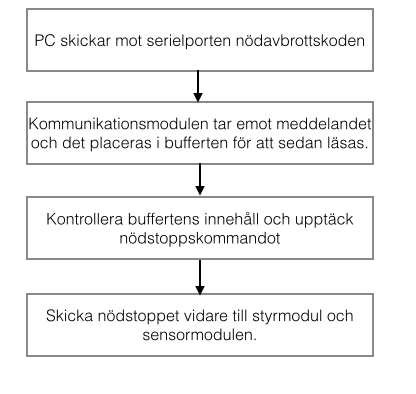
\includegraphics[keepaspectratio=true,width=0.5\linewidth]{bilder/SPIbild005.jpg}  %skala och filnamn. 
  \end{center}
  \caption{Flödesdiagram för Fall 4.} %figurtext.
  \label{fig:case4flow}
\end{figure}
\thispagestyle{empty}

\end{document}